% Requires XeLaTeX to process
\documentclass[t]{beamer}
\usepackage{media9}
\usepackage{graphicx}
\usepackage{siunitx}
\sisetup{load-configurations = abbreviations}

\mode<presentation> {
  \usetheme{boxes}
  \usecolortheme{rose}
  \setbeamertemplate{navigation symbols}{} % To remove the navigation symbols from the bottom of all slides uncomment this line
}

%\usepackage{pgfpages}
%\pgfpagesuselayout{2 on 1}[a4paper,border shrink=5mm]

\usefonttheme[onlymath]{serif}
\usepackage{fontspec} 
\defaultfontfeatures{Mapping=tex-text} 
\setsansfont[Ligatures={Common}]{Futura}
\setmonofont[Scale=0.8]{Monaco} 

\usepackage{graphicx} % Allows including images
\usepackage{booktabs} % Allows the use of \toprule, \midrule and \bottomrule in tables

%----------------------------------------------------------------------------------------
% New Commands
%----------------------------------------------------------------------------------------

\newcommand*{\movie}[1]{\includemedia[width=0.6\linewidth,height=0.3375\linewidth, activate=pageopen]{}{#1}}
\newcommand{\img}[1]{\includegraphics[width=1\linewidth]{images/#1}}
\newcommand{\imgs}[1]{\includegraphics[width=.75\linewidth]{images/#1}}
\newcommand{\imgss}[1]{\includegraphics[width=.5\linewidth]{images/#1}}
\newcommand{\bi}{\begin{itemize}}
\newcommand{\ei}{\end{itemize}}

%----------------------------------------------------------------------------------------
%	TITLE PAGE
%----------------------------------------------------------------------------------------
\title[Topic 4]{Grade 8 - Light and Optics} % The short title appears at the bottom of every slide, the full title is only on the title page
\subtitle{Topic 4: Lenses and vision}
\author{Dr. Pineda} 
\institute[] {\href{http://www.drpineda.ca}{www.drpineda.ca}}
\date{} % Date, can be changed to a custom date

% Customize the footline
%\setbeamertemplate{footline}{goo \insertframenumber \insertsubtitle \inserttitle}

\setbeamertemplate{footline}{
   \begin{beamercolorbox}[ht=4ex,leftskip=.2cm,rightskip=.2cm]{author in head/foot}
    \usebeamercolor{UniBlue}
    \hrule
    \vspace{0.1cm}
    \inserttitle \ - \insertsubtitle \hfill \insertframenumber/\inserttotalframenumber
   \end{beamercolorbox}
   \vspace*{0.1cm}
} 

%----------------------------------------------------------------------------------------
%	BEGIN DOCUMENT
%----------------------------------------------------------------------------------------
\begin{document}

{
\setbeamertemplate{footline}{} % no page number here
\frame{\titlepage}
}

%----------------------------------------------------------------------------------------
%	PRESENTATION SLIDES
%----------------------------------------------------------------------------------------

%----------------------------------------------------------------------------------------
%	Refraction
%----------------------------------------------------------------------------------------
\begin{frame}{Refraction}
\bi
\item The bending of light when it travels from one medium to another. 
\item The speed of light changes slightly when it moves through materials of different densities.  
\item The denser the material, the slower light goes. 
\item It makes objects appear in different positions. 
\ei
\end{frame}

\begin{frame}
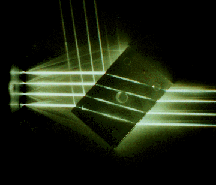
\includegraphics[width=1\linewidth]{images/refraction.png}
\end{frame}

\end{document}